\chapter{Desarrollo de la Web Actual}
\label{desarrolloWeb}
\section{Introducci'on}

Internet es la interconexi'on global de redes individuales alrededor del mundo. Originalmente fu'e utilizada para interconectar laboratorios dedicados a investigaci'on gubernamental. Desde 1994 se expandi'o para millones de usuarios de todo el mundo que la utilizan con m'ultiples prop'ositos. A medida que iba creciendo, cambiaba la forma de hacer negocios y de comunicarse. Hasta llegar a ser una fuente de informaci'on Universal para millones de personas \citep{iws}.

Internet contin'ua creciendo d'ia a d'ia. Hacia 1995 la cantidad de usuarios promedio era de 16 millones, 1 a'no despu'es, la cifra ascendi'o a m'as del doble. Para el a�o 2000 se increment'o 10 veces la cantidad de usuarios. Esta informaci'on puede verse en el Cuadro \ref{cuadroCrecInternet}.

\begin{longtable}{l c c}
\hline
 Fecha & Usuarios(mill) & \% Poblaci'on Mundial\\
\hline \hline
\endfirsthead

\hline
 Fecha & Usuarios(mill) & \% Poblaci'on Mundial\\
\hline \hline
\endhead

\multicolumn{3}{l}{Sigue en la p'agina siguiente.}
\endfoot

\endlastfoot

\hline
Diciembre, 1995 & 16 & 0.4 \\
Diciembre, 1996 & 36 & 0.9 \\
Diciembre, 1997 & 70 & 1.7 \\
Diciembre, 1998 & 147 & 3.6 \\
Diciembre, 1999 & 248 & 4.1 \\
Diciembre, 2000 & 361 & 5.8 \\
Agosto, 2001 & 513 & 8.6 \\
Septiembre, 2002 & 587 & 9.4 \\
Diciembre,  2003 & 719 & 11.1 \\
Diciembre,  2004 & 817 & 12.7 \\
Diciembre,  2005 & 1018 & 15.7 \\
Diciembre, 2006 & 1093 & 16.7 \\
Diciembre, 2007 & 1319 & 20.0 \\
Diciembre, 2008 & 1574 & 23.5 \\
Marzo, 2009 & 1596 & 23.8 \\
Junio, 2009 & 1669 & 24.7 \\
Septiembre, 2009 & 1734 & 25.6 \\
Diciembre, 2009 & 1802 & 26.6 \\
Junio, 2010 & 1966 & 28.7 \\
Septiembre, 2010 & 1971 & 28.8 \\
Marzo, 2011 & 2095 & 30.2 \\
Junio, 2011 & 2110 & 30.4 \\
Septiembre, 2011 & 2180 & 31.5 \\
Diciembre, 2011 & 2267 & 32.7 \\
Marzo, 2012 & 2336 & 33.3 \\
Junio, 2012 & 2405 & 34.3 \\
Septiembre, 2012 & 2439 & 34.8 \\
Diciembre, 2012 & 2497 & 35.7 \\
Marzo, 2013 & 2749 & 38.8 \\
\hline
\caption{Crecimiento de la cantidad de usuarios de Internet, informaci'on extra'ida de \cite{iws}}
\label{cuadroCrecInternet}
\end{longtable}

Tambi'en puede observarse en el Gr'afico \ref{grafCrecInternet} el incre'ible crecimiento que tuvo la cantidad de usuarios de Internet, y es clara la tendencia de seguir creciendo.

\begin{figure}[h]
  	\centering
	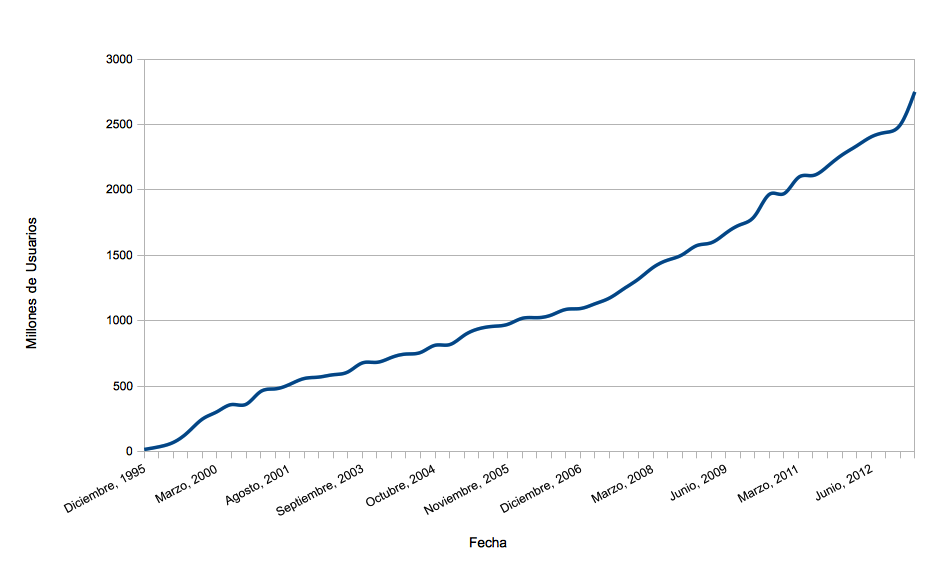
\includegraphics[width=\textwidth]{img/grafCrecInternet}
	\caption{\small Crecimiento de la cantidad de usuarios de Internet, informaci'on extra'ida de \cite{iws}}
	\label{grafCrecInternet}
\end{figure}

Adem'as de la cantidad de usuarios, en paralelo iba creciendo la cantidad de Dominios. En sus inicios, la cantidad de dominios era de 19.732 (medici'on realizada en Agosto de 1995), la medici'on m'as actual (Febrero 2014) realizada por Netcraft\footnote{NetCraft - http://news.netcraft.com/} da un total aproximado de sitios de 920.102.079 \citep{netcraft} (58 millones m'as que el mes anterior). Esto se puede ver en el Gr'afico \ref{grafNetcraft}.

\begin{figure}[h]
  	\centering
	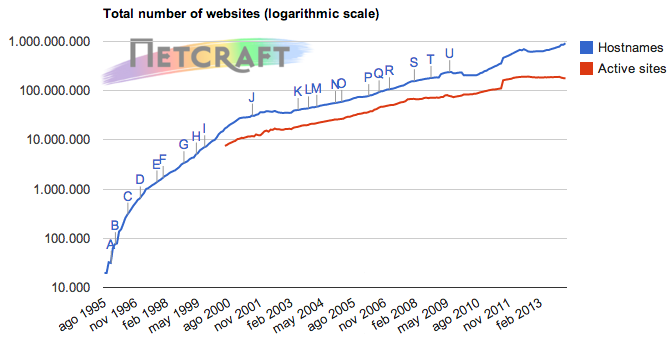
\includegraphics[width=\textwidth]{img/grafNetcraft}
	\caption{\small Crecimiento de la cantidad de sitios en Internet, extra'ido de \cite{netcraft}}
	\label{grafNetcraft}
\end{figure}

Tambi'en fu'e aumentando el tama'no promedio de los sitios as'i tambi'en como la cantidad de recursos que poseen los mismos. En el a�o 1997, el tama�o promedio de un sitio era de 60Kb \citep{atw}, pr'acticamente era todo texto, pocas im'agenes y poca interactividad. Esto fu'e cambiando con el tiempo, con el avance de la tecnolog'ia y de los recursos que se pod'ian compartir en la red. El crecimiento a lo largo del tiempo puede verse en el Gr'afico \ref{grafCrecSitios}

\begin{figure}[h]
  	\centering
	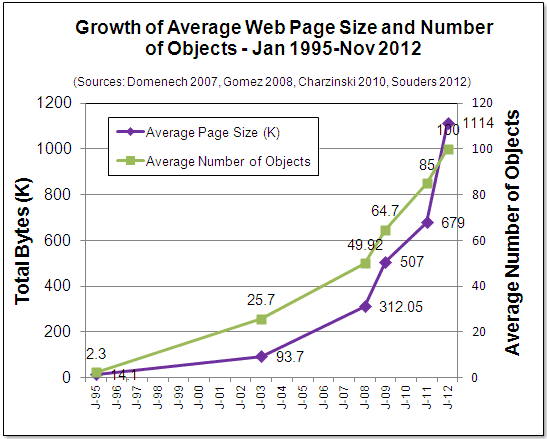
\includegraphics[width=\textwidth]{img/grafCrecSitios}
	\caption{\small Crecimiento del tama'no de los sitios en Internet (1995 a 2012), extra'ido de \cite{tamanoSitios}}
	\label{grafCrecSitios}
\end{figure}

Actualmente, el promedio es de 1687Kb\footnote{Medici'on extra'ida de \citep{httparchive} el 1 de Febrero 2014}, su contenido es mucho m'as variado e interactivo. Hoy los sitios se componen de diversos tipos de recursos, scripts, hojas de estilo, diferentes tipos de im'agenes, video, contenido Flash\footnote{http://www.adobe.com/}, etc. El promedio detallado por contenido de los sitios se pueden ver en el Gr'afico \ref{grafSitiosFeb2014}

\begin{figure}[h]
  	\centering
	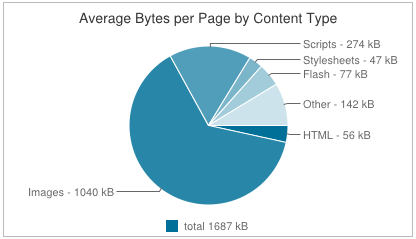
\includegraphics[width=\textwidth]{img/grafSitiosFeb2014}
	\caption{\small Tama'no promedio de los sitios en Internet, detallado por contenido, extra'ido de \cite{httparchive}}
	\label{grafSitiosFeb2014}
\end{figure}


FALTA: UTILIZACION HTTP HTTPS